%%% Local Veriables:
%%% coding: utf-8
%%% mode: latex
%%% TeX-engine: xetex
%%% End:

\documentclass{article}
\usepackage{latexsym}
\usepackage{amsmath}
\usepackage{amssymb}

\usepackage[top=1.25in, bottom=1.25in, left=1.5in, right=1.5in]{geometry}

\usepackage{xeCJK}
\usepackage{fontspec,xltxtra,xunicode}
\setCJKmainfont[ItalicFont=KaiTi, BoldFont=SimHei]{SimSun}
\setCJKsansfont{SimHei}
\setCJKmonofont{FangSong}

\newcommand{\song}{\CJKfamily{SimSun}}
\setCJKfamilyfont{fs}{FangSong}
\newcommand{\fs}{\CJKfamily{fs}}
\setCJKfamilyfont{kai}{KaiTi}
\newcommand{\kai}{\CJKfamily{kai}}
\setCJKfamilyfont{yahei}{Microsoft YaHei}
\newcommand{\yahei}{\CJKfamily{yahei}}
\setCJKfamilyfont{hei}{SimHei}
\newcommand{\hei}{\CJKfamily{hei}}
\setCJKfamilyfont{lishu}{LiSu}
\newcommand{\lishu}{\CJKfamily{lishu}}
\setCJKfamilyfont{youyuan}{YouYuan}
\newcommand{\youyuan}{\CJKfamily{youyuan}}

\usepackage{algorithm}
\usepackage{algorithmic}

\usepackage{graphicx}
\usepackage{hyperref}

\begin{document}
\author{BYIII}
\title{Quaternion, Euler Angles, and Rotation Matrix}
\date{}

\maketitle

\section{Quaternion}

The quaternion is a number system that extends the complex numbers. Quaternion was first introduced by Irish mathematician William Rowan Hamilton in 1843.

Complex numbers have one imaginary part, which is often denoted as $i$. Quaternions extend to three imaginary parts, $i$, $j$, and $k$. Formally, a quaternion is a four-dimensional vector space over the real number. The quaternions set \textbf{H} has three operations: addition, scalar multiplication, and quaternion multiplication.

%% ************************************
\subsection{Multiplication of Basic Elements}

Firstly, and most importantly, the multiplication of basic elements of quaternions:
\begin{equation}
  \begin{split}
    i^2 &= -1, \\
    j^2 &= -1, \\
    k^2 &= -1, \\
    ijk &= -1.
  \end{split}
\end{equation}
where $i$, $j$, $k$ denote the basis elements of the imaginary part of \textbf{H}. And from the above definition, we can derive:
\begin{equation}
  \begin{split}
    ij = k, &\quad ji = -k, \\
    jk = i, &\quad kj = -i, \\
    ki = j, &\quad ik = -j.
  \end{split}
\end{equation}

Then, we should notice that the multiplication between quaternions is not commutative. And the multiplication between two of imaginary bases $i$, $j$, $k$ following the \textit{i->j->k->i->...} order loop will result in a positive of the missing one, if not, then the negative of the missing imaginary basis.

%% ***********
\subsection{Addition}

The Addition between two quaternions $q_1 = a_1 + ib_1+jc_1+kd_1$ and $q_2 = a_2 + ib_2+jc_2+kd_2$ is just the same as the linear vector space:
\begin{equation}
  q_1 + q_2 = (a_1+a_2) + i(b_1+b_2) + j(c_1+c_2) + k(d_1+d_2).
\end{equation}

%% ************************
\subsection{Scalar Multiplication}

A scalar number multiplies a quaternion is same as the scalar multiplication operation in the linear vector space. If $s$ is the scalar, and $q=a+ib+jc+kd$, then the scalar multiplication s*q is:
\begin{equation}
  s*q =  as+ibs+jcs+kds.
\end{equation}

%% ****************************
\subsection{Hamilton Product}

The product of two quaternions, $q_1=a_1+ib_1+jc_1+dk_1$ and $q_2=a_2+ib_2+jc_2+kd_2$, is called the Hamilton product. Due to the non-commutativity of multiplication of the basic elements, the Hamilton product is different from the complex number product:
\begin{equation}
  \begin{split}
    q_1q_2 &= (a_1+ib_1+jc_1+kd_1)(a_2+ib_2+jc_2+kd_2) \\
    &= a_1a_2+ia_1b_2+ja_1c_2+ka_1d_2             \\
    &\quad +ib_1a_2+i^2b_1b_2+ijb_1c_2+ikb_1d_2   \\
    &\quad +jc_1a_2+jic_1b_2+j^2c_1c_2+jkc_1d_2   \\
    &\quad +kd_1a_2+kid_1b_2+kjd_1c_2+k^2d_1d_2   \\
    &= a_1a_2-b_1b_2-c_1c_2-d_1d_2                \\
    &\quad +i(a_1b_2+b_1a_2+c_1d_2-d_1c_2)         \\
    &\quad +j(a_1c_2-b_1d_2+c_1a_2+d_1b_2)         \\
    &\quad +k(a_1d_2+b_1c_2-c_1b_2+d_1a_2)         \\
    & = \begin{pmatrix}
      a_1a_2-b_1b_2-c_1c_2-d_1d_2         \\
      a_1b_2+b_1a_2+c_1d_2-d_1c_2         \\
      a_1c_2-b_1d_2+c_1a_2+d_1b_2         \\
      a_1d_2+b_1c_2-c_1b_2+d_1a_2         \\
    \end{pmatrix}.
  \end{split}
\end{equation}

%% **************
\subsection{Conjugation}

The conjugation of a quaternion $p=a+ib+jc+kd$ is 
\begin{equation}
  q^*=a-ib-jc-kd. 
\end{equation}
It is the same with the complex number. Specially, the quaternion conjugation can be represented by multiplication as addition:

\begin{equation}
  q^* = -1/2(q+iqi+jqj+kqk).
\end{equation}

Conjugation is an involution, meaning that it is its own inverse, so conjugating an element twice returns the original element. And the conjugation of a product of two quaternion is:
\begin{equation}
  (pq)^* = q^*p^*.
\end{equation}
That is similar to that of two element in the common linear vector space.

%% ******************
\subsection{Quaternion Norm}

Notice that the Hamilton product of a quaternion and its conjugation is a real number, or we say the product has zero imaginary part. The norm of a quaternion is defined as:

\begin{equation}
  \|q\| = \sqrt{qq^*} = \sqrt{q^*q} = \sqrt{a^2+b^2+c^2+d^2}
\end{equation}

Two properties of quaternion norm:
\begin{equation}
  \begin{split}
    \|sq\| &= |s| \cdot \|q\|   \\
    \|pq\| &= \|p\| \cdot \|q\|
  \end{split}
\end{equation}

%% *********************************
\subsection{Unit Quaternion and Reciprocal}
The unit quaternion is a quaternion whose norm is 1. That is:
\begin{equation}
  U_q = \frac{q}{\|q\|}
\end{equation}
Based on the conjugation and the norm, the reciprocal of a quaternion is another quaternion that the Hamilton product of them is equal to 1:
\begin{equation}
  q^{-1} = \frac{1}{\|q\|^2}
\end{equation}

%% ****************************************
\section{Quaternion and Spatial Rotation in $\mathbb{R}^3$}

%% *************************************
\subsection{Quaternion and the Geometry of $\mathbb{R}^3$}

We can divide a quaternion in to scalar part and imaginary part: $p = s+v$, s is a scalar, and $v$ is a vector in $\mathbb{R}^3$. Because the vector part of a quaternion is a vector in $\mathbb{R}^3$, the geometry of $\mathbb{R}^3$ is reflected in the algebraic structure of the quaternions. Many operations on vectors can be defined in terms of quaternions, and this makes it possible to apply quaternion techniques wherever spatial vectors arise. For instance, this is true in electrodynamics and 3D computer graphics.

Set two pure imaginary quaternions $p = ib_1+jc_1+kd_1$, and $q = ib_2+jc_2+kd_2$. Their dot product is
\begin{displaymath}
  p \cdot q = b_1b_2+c_1c_2+d_1d_2
  = \frac{1}{2}(p^*q+q^*p) = \frac{1}{2}(pq^*+qp^*)
\end{displaymath}
The cross product of p and q is:
\begin{displaymath}
  p \times q = i(c_1d_2-d_2c_1)+j(d_1b_2-b_1d_2)+k(b_1c_2-c_1b_2)
  =\frac{1}{2}(pq-q^*p^*)
\end{displaymath}

In general, let $p$ and $q$ be quaternioins:
\begin{displaymath}
  \begin{split}
    p = s_1+v_1,
    q = s_2+v_2.
  \end{split}
\end{displaymath}
Then the Hamilton product of $p$ and $q$ can be written as:
\begin{displaymath}
  pq = (s_1s_2-v_1 \cdot v_2)+(s_1v_2+s_2v_1+v_1 \times v_2).
\end{displaymath}

\subsection{Spatial Rotation in $\mathbb{R}^3$}
Any rotation in 3-dimensions can be represented as a combination of a vector $\mathbf{u}$ and a scalar $\theta$. Quaternion offers a simple way to encode this axis-angle representation in four numbers, and can be used to apply the corresponding rotation to a position vector. A rotation through an angle of $\theta$ around the axis defined by a unit vector:
\begin{displaymath}
  \mathbf{u} = (u_x, u_y, u_z) = iu_x + ju_y + ku_z
\end{displaymath}
can be represented by a unit quaternion:
\begin{equation}
  q = e^{\frac{\theta}{2}(iu_x+ju_y+ku_z)} = \cos{\frac{\theta}{2}}+(iu_x+ju_y+ku_z)\sin{\frac{\theta}{2}}
\end{equation}

A point in 3-dimensional space can be expressed with quaternion: $v = 0+ib+jc+kd$. Then applying the rotation to this point is to the following Hamilton production:
\begin{equation}
  v' = qvq^{-1} = qvq^*.
\end{equation}
Notice that $\|q\| = 1$, so $q^-1 = q^*/\|q\|^2 = q^*$. If $p$ and $q$ are unit quaternions, then rotation by $pq$ is
\begin{displaymath}
  pqv(pq)^{-1} = pqvq^{-1}p^{-1} = p(qvq^{-1})p^{-1},
\end{displaymath}
which is the same as rotating (conjugating) by $q$ and then by $p$. From $v' = qvq^{-1}$ to compute the rotation matrix:
\begin{displaymath}
  \begin{aligned}
    v' &= ip_x'+jp_y'+kp_z' \\
    &= \begin{pmatrix}
      \cos{theta/2}     \\
      u_x\sin{\frac{\theta}{2}}  \\
      u_y\sin{\frac{\theta}{2}}  \\
      u_z\sin{\frac{\theta}{2}}
    \end{pmatrix}\begin{pmatrix}
      0 \\p_x \\ p_y \\p_z 
    \end{pmatrix} \begin{pmatrix}
      \cos{\frac{\theta}{2}}      \\
      -u_x\sin{\frac{\theta}{2}}  \\
      -u_y\sin{\frac{\theta}{2}}  \\
      -u_z\sin{\frac{\theta}{2}}
    \end{pmatrix} \\
    &= \begin{pmatrix}
      -u_xp_x\sin{\frac{\theta}{2}}-u_yp_y\sin{\frac{\theta}{2}}-u_zp_z\sin{\frac{\theta}{2}} \\
      (p_x\cos{\frac{\theta}{2}}+u_yp_z\sin{\frac{\theta}{2}}-p_yu_z\sin{\frac{\theta}{2}})  \\
      (p_y\cos{\frac{\theta}{2}}-u_xp_z\sin{\frac{\theta}{2}}-u_zp_x\sin{\frac{\theta}{2}})  \\
      (p_z\cos{\frac{\theta}{2}}+u_xp_y\sin{\frac{\theta}{2}}-u_yp_x\sin{\frac{\theta}{2}})
    \end{pmatrix}\begin{pmatrix}
      \cos{theta/2}  \\
      -u_x\sin{\frac{\theta}{2}}  \\
      -u_y\sin{\frac{\theta}{2}}  \\
      -u_z\sin{\frac{\theta}{2}}
    \end{pmatrix} \\
    &= \begin{pmatrix} 0 \\
      p_x(\cos^2{\frac{\theta}{2}}+u_x^2\sin^2{\theta}-u_y^2\sin^2{\frac{\theta}{2}}-u_z^2\sin^2{\frac{\theta}{2}}) \\
      \cdots \\ \cdots \end{pmatrix} 
    + \begin{pmatrix}
      0 \\
      p_y(2u_xu_y\sin^2{\frac{\theta}{2}}-2u_z\sin{\frac{\theta}{2}}\cos{\frac{\theta}{2}}) \\
      \cdots \\ \cdots \end{pmatrix} \\
    & \quad + \begin{pmatrix} 0 \\
      p_z(2u_xu_z\sin{\frac{\theta}{2}}+2u_y\sin{\frac{\theta}{2}}\cos{\frac{\theta}{2}})  \\
      \cdots \\ \cdots \end{pmatrix}
  \end{aligned}
\end{displaymath}

Then then rotation matrix for a unit quaternion $q = q_0 + iq_1 + jq_2 + kq_3$ is:
\begin{equation}
  R = \begin{bmatrix}
    1-2q_2^2-2q_3^2 & 2(q_1q_2-q_3q_0)  & 2(q_1q_3+q_2q_0)  \\
    2(q_1q_2+q_3q_0)  & 1-2q_1^2-2q_3^2 & 2(q_2q_3-q_1q_0)  \\
    2(q_1q_3-q_2q_0)  & 2(q_2q_3+q_1q_0)  & 1-2q_1^2-2q_2^2
  \end{bmatrix}
\end{equation}

Further more, the conversion from rotation matrix to quaternion is:
\begin{displaymath}
  \text{assume } R = \begin{bmatrix}
    r_{11} & r_{12} & r_{13} \\
    r_{21} & r_{22} & r_{23} \\
    r_{31} & r_{32} & r_{33}
  \end{bmatrix},
\end{displaymath}
then the corresponding quaternion $q = q_0+iq_1+jq_2+kq_3$ can be decomposed as:
\begin{equation}
  \begin{split}
    q_0 &= \frac{\sqrt{tr(R)+1}}{2},    \\
    q_1 &= \frac{r_{32}-r_{23}}{4q_0}, \\
    q_2 &= \frac{r_{13}-r_{31}}{4q_0}, \\
    q_3 &= \frac{r_{21}-r_{12}}{4q_0}
  \end{split}
\end{equation}
if $q_0$ is not equal to zero. Otherwise, we should use the rotation matrix to axis-angle decomposition to calculate the quaternion.

%% **************
\section{Euler Angles}

Very very brief here...

Without considering the possibility of using two different conventions for the definition of the rotation axes (intrinsic or extrinsic), there exist twelve possible sequences of rotation axes, divided in two groups:

\begin{itemize}
\item Proper Euler angles (z-x-z, x-y-x, y-z-y, z-y-z, x-z-x, y-x-y),
\item Tait–Bryan angles (x-y-z, y-z-x, z-x-y, x-z-y, z-y-x, y-x-z).
\end{itemize}


%% **********************************************
\subsection{Intrinsic Rotations and Extrinsic Rotations}

\subsubsection*{Intrinsic Rotations}

Intrinsic rotations are rotations that the rotating axis system is fixed with the rotating object. For example, for the rotation sequence x-y'-z'':

\begin{itemize}
\item At the initial time, the rotation axis system x0-y0-z0 is identity with X-Y-Z, 
\item we first rotate about the x0 axis, the object-fixed rotation system is also rotated, denoted as x1-y1-z1,
\item then we rotate about the y1 axis, the rotation system is then x2-y2-z2,
\item and finally rotate about the z2 axis.
\end{itemize}

Intrinsic rotation matrix represents the transformation from axis system x2-y2-z2 to axis system x0-y0-z0.

\subsubsection*{Yaw, Pitch and Roll}

Yaw, pitch and roll are the three rotation angle corresponding to the intrinsic rotation in the sequence of z-y'-x''.

\subsubsection*{Extrinsic Rotations}

Extrinsic rotations are rotations that the rotating axis system is the fixed world axis system X-Y-Z. And the rotation matrix represents the transformation from before the rotation the after the rotation.

%% **********************************
\section{Euler Angles and Rotation Matrix}

\subsection{From Euler Angles to Rotation Matrix}

Assume we know the extrinsic rotation Euler angles $[\psi, \theta, \phi]$ in the rotation sequence x-y-z. Then the rotation matrix can be computed as:

\begin{eqnarray}
    Rx(\psi) &= \begin{bmatrix}
      1 & 0          & 0           \\
      0 & \cos{\psi} & -\sin{\psi} \\
      0 & \sin{\psi} & \cos{\psi}
    \end{bmatrix} \\
    Ry(\theta) &= \begin{bmatrix}
      \cos{\theta}  & 0 & \sin{\theta} \\
      0             & 1 & 0            \\
      -\sin{\theta} & 0 & \cos{\theta}
    \end{bmatrix} \\
    Rz(\phi) &= \begin{bmatrix}
      \cos{\phi} & -\sin{\phi} & 0 \\
      \sin{\phi} & \cos{\phi}  & 0 \\
      0          &  0          & 1
    \end{bmatrix}
\end{eqnarray}

\begin{equation}
  \begin{split}
    R &= Rz(\phi)Ry(\theta)Rx(\psi) \\
    &= \begin{bmatrix}
      \cos{\theta}\cos{\phi} & \sin{\psi}\sin{\theta}\cos{\phi}−\cos{\psi}\sin{\phi} & \cos{\psi}\sin{\theta}\cos{\phi}+\sin{\psi}\sin{\phi} \\
      \cos{\theta}\sin{\phi} & \sin{\psi}\sin{\theta}\sin{\phi}+\cos{\psi}\cos{\phi} & \cos{\psi}\sin{\theta}\sin{\phi}−\sin{\psi}\cos{\phi} \\
      −\sin{\theta}          & \sin{\psi}\cos{\theta}                                & \cos{\psi}\cos{\theta}
    \end{bmatrix}
  \end{split}
\end{equation}


\subsection{The Decomposition of Euler angles from Rotation Matrix}
\begin{center}\begin{minipage}[c]{0.7\linewidth}
\begin{algorithm}[H]
\begin{algorithmic}
  \IF{$r_{31} != ±1$}
    \STATE $\theta_1 = −\text{asin}(r_{31})$
    \STATE $\theta_2 = \pi − \theta_1$
    \STATE $\psi_1 = \text{atan2}(r_{32}/\cos{\theta_1}, r_{33}/\cos{\theta_1})$
    \STATE $\psi_2 = \text{atan2}(r_{32}/\cos{\theta_2}, r_{33}/\cos{\theta_2})$
    \STATE $\phi_1 = \text{atan2}(r_{21}/\cos{\theta_1}, r_{11}/\cos{\theta_1})$
    \STATE $\phi_2 = \text{atan2}(r_{21}/\cos{\theta_2}, r_{11}/\cos{\theta_2})$
  \ELSE
    \STATE $\phi = \text{anything}$; can set to 0,
    \IF{$R_{31} = −1$}
      \STATE $\theta = \frac{\pi}{2}$
      \STATE $\psi = \phi + \text{atan2}(r_{12}, r_{13})$
    \ELSE
      \STATE $\theta = −\pi/2$
      \STATE $\psi = −\phi + \text{atan2}(−r_{12}, −r_{13})$
    \ENDIF
  \ENDIF
\end{algorithmic}
\caption{Extracting Euler angles from rotation matrix}
\label{alg:a1}
\end{algorithm}
\end{minipage}
\end{center}

Algorithm \ref{alg:a1} lists the procedure to extract Euler angles from a rotation matrix. In both the $\theta=\pi/2$ and $\theta=−\pi/2$ cases, we have found that $\psi$ and $\phi$ are linked. This phenomenon is called Gimbal lock. In the normal case($\theta \ne \pm \pi/2$), there are two sets of result, then we can just assume that $\theta$ lies in $[-\pi/2, \pi/2]$ to solve the ambiguity.


%% ******************************
\section{Euler Angles and Quaternions}

According to the relationship between unit quaternion and rotations in three dimensional space, the squencial rotation around the fixed world axis system $x-\psi$, $y-\theta$, and $z-\phi$ can be written as:

\begin{displaymath}
\begin{split}
  q =& q_zq_yq_x, \\
  &q_x = \begin{pmatrix} \cos{\psi/2} \\
  \sin{\psi/2} \\ 0 \\ 0 \end{pmatrix}, \,
  q_y = \begin{pmatrix} \cos{\theta/2} \\
  0 \\ \sin{\theta/2} \\ 0 \end{pmatrix}, \,
  q_z = \begin{pmatrix} \cos{\phi/2} \\
  0 \\ 0 \\ \sin{\phi/2} \end{pmatrix}
\end{split}
\end{displaymath}

\begin{equation}
  q = \begin{pmatrix}
    \cos{\psi/2}\cos{\theta/2}\cos{\phi/2}+\sin{\psi/2}\sin{\theta/2}\sin{\phi/2} \\
    \sin{\psi/2}\cos{\theta/2}\cos{\phi/2}-\cos{\psi/2}\sin{\theta/2}\sin{\phi/2} \\
    \cos{\psi/2}\sin{\theta/2}\cos{\phi/2}+\sin{\psi/2}\cos{\theta/2}\sin{\phi/2} \\
    \cos{\psi/2}\cos{\theta/2}\sin{\phi/2}-\sin{\psi/2}\sin{\theta/2}\cos{\phi/2}
  \end{pmatrix}
\end{equation}

Now we can extract Euler angles base on the above equation:
\begin{itemize}
\item in case that $\theta \ne \pm \pi/2$: 
\begin{equation}%
\begin{aligned}%
  \psi   &= \text{atan}\left(\frac{2(q_0q_1+q_2q_3)}{1-2*(q_1^2+q_2^2)}\right) \\
  \theta &= \text{asin}\left(2(q_0q_2-q_3q_1) \right)                   \\
  \phi   &= \text{atan}\left(\frac{2(q_0q_3+q_1q_2)}{1-2*(q_2^2+q_3^2}\right)
\end{aligned}%
\end{equation}

\item in case that $\theta = \pi/2$ :
\begin{equation}
q = \frac{\sqrt{2}}{2}\begin{pmatrix}%
\cos{\psi/2}\cos{\phi/2}+\sin{\psi/2}\sin{\phi/2} \\
\sin{\psi/2}\cos{\phi/2}-\cos{\psi/2}\sin{\phi/2} \\
\cos{\psi/2}\cos{\phi/2}+\sin{\psi/2}\sin{\phi/2} \\
\cos{\psi/2}\sin{\phi/2}-\sin{\psi/2}\cos{\phi/2}
\end{pmatrix}
\end{equation}
then we can get:
\begin{displaymath}
\begin{aligned}
  \tan{\left(\frac{\phi}{2}-\frac{\psi}{2}\right)} = \frac{q_1}{q_0} \\
\phi = \psi + 2\, \text{atan2}(q_1, q_0) \\
\psi = \phi - 2\, \text{atan2}(q_1, q_0)
\end{aligned}
\end{displaymath}
so Euler angles is:
\begin{equation}%
\begin{aligned}%
\psi &= \phi - 2\, \text{atan2}(q_1, q_0) \\
\theta &= \frac{\pi}{2} \\
\phi &= \text{anything, can set to 0}
\end{aligned}%
\end{equation}

\item in case that $\theta = -\pi/2$ :
\begin{equation}
q = \frac{\sqrt{2}}{2}\begin{pmatrix}%
\cos{\psi/2}\cos{\phi/2}-\sin{\psi/2}\sin{\phi/2} \\
\sin{\psi/2}\cos{\phi/2}+\cos{\psi/2}\sin{\phi/2} \\
-\cos{\psi/2}\cos{\phi/2}+\sin{\psi/2}\sin{\phi/2} \\
\cos{\psi/2}\sin{\phi/2}+\sin{\psi/2}\cos{\phi/2}
\end{pmatrix}
\end{equation}
then we can get:
\begin{displaymath}
\begin{aligned}
  \tan{\left(\frac{\phi}{2}+\frac{\psi}{2}\right)} = \frac{q_1}{q_0} \\
\phi = -\psi + 2\, \text{atan2}(q_1, q_0) \\
\psi = -\phi + 2\, \text{atan2}(q_1, q_0)
\end{aligned}
\end{displaymath}
so Euler angles is:
\begin{equation}%
\begin{aligned}%
\psi &= -\phi + 2\, \text{atan2}(q_1, q_0) \\
\theta &= -\frac{\pi}{2} \\
\phi &= \text{anything, can set to 0}
\end{aligned}%
\end{equation}

\end{itemize}


\section{Inverse Trigonometric Functions in C++}
\begin{itemize}
\item $\alpha = \text{asin}(x)$: $x \in [-1, 1] \to \alpha \in [-\pi/2, \pi/2]$;

\item $\alpha = \text{acos}(x)$: $x \in [-1, 1] \to \alpha \in [0, \pi]$;

\item $\alpha = \text{atan}(x)$: 
\begin{displaymath}
\begin{aligned}
x \in (-\infty,\infty) &\to \alpha \in (-\pi/2, \pi/2) \\
x = \pm 0 &\to \alpha = 0 \\
x = +\infty &\to \alpha = \pi/2 \\
x = -\infty &\to \alpha = -\pi/2
\end{aligned}
\end{displaymath}

\item $\alpha = \text{atan2}(y, x)$, same as $\alpha = \tan{\frac{y}{x}}$: \\
\centerline{$y,x \in (-\infty,\infty) \to \alpha \in [-\pi, \pi]$}
\begin{itemize}
\item If x and y are both zero, domain error does not occur
\item If x and y are both zero, range error does not occur either
\item If y is zero, pole error does not occur
\item If y is $\pm 0$ and x is negative or -0, $\pm \pi$ is returned
\item If y is $\pm 0$ and x is positive or +0, $\pm 0$ is returned
\item If y is $\pm \infty$ and x is finite, $\pm \pi/2$ is returned
\item If y is $\pm \infty$ and x is $-\infty$, ±3π/4 is returned
\item If y is $\pm \infty$ and x is $+\infty$, ±π/4 is returned
\item If x is $\pm 0$ and y is negative, $-\pi/2$ is returned
\item If x is $\pm 0$ and y is positive, $+\pi/2$ is returned
\item If x is $-\infty$ and y is finite and positive, $+\pi$ is returned
\item If x is $-\infty$ and y is finite and negative, $-\pi$ is returned
\item If x is $+\infty$ and y is finite and positive, +0 is returned
\item If x is $+\infty$ and y is finite and negative, -0 is returned
\item If either x is NaN or y is NaN, NaN is returned
\end{itemize}
\end{itemize}

\begin{figure}[!ht]
\centering
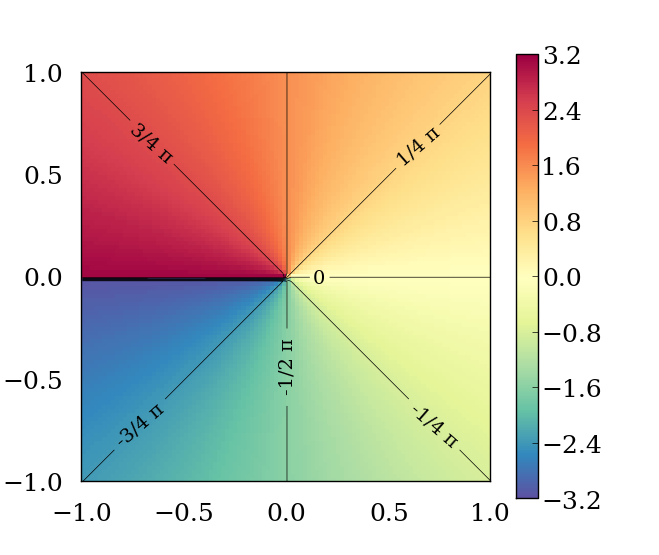
\includegraphics[width=3in]{figures/atan2.png}
\caption{atan2 function domain and region}
\label{fig:atan2}
\end{figure}


%% ***********
\begin{thebibliography}{99}
\bibitem{blog} 视觉SLAM中的数学基础,第二篇,四元数. \url{http://www.cnblogs.com/gaoxiang12/p/5120175.html}.
\bibitem{WikiQ} Wikipedia. Quaternion. \url{https://en.wikipedia.org/wiki/Quaternion}.
\bibitem{WikiQS} Wikipedia. Quaternion and Spatial Rotation. \url{https://en.wikipedia.org/wiki/Quaternions_and_spatial_rotation}.
\bibitem{WikiE} Wikipedia. Euler Angles. \url{https://en.wikipedia.org/wiki/Euler_angles}.
\bibitem{WikiC} Wikipedia. Conversion Between Quaternions and Euler Angles. \url{https://en.wikipedia.org/wiki/Conversion_between_quaternions_and_Euler_angles}.
\bibitem{Gregory} Gregory G. Slabaugh. Computing Euler angles from a rotation matrix.
\end{thebibliography}

\end{document}
